\chapter{The Standard Model}
\label{c:the_standard_model}

The top quark was discovered by the CDF and D{\O} collaborations in 1995 and is still one of the less
well studied fundamental particles in the Standard Model. The top quark is the heaviest fermion with its mass
currently placed at $173.29 \pm 0.23 (stat.) \pm 0.92 (syst.)~GeV/c^{2}$ \cite{top_mass}. Since the lifetime
of the top quark is very short, approximately $5 \times 10^{25}~s$, it is the only one of the quarks to decay
before it hadronises, meaning that the bare quark properties can be investigated. These unique properties of
the top quark within the Standard Model mean it is an interesting focus of study.

During 2011 and 2012, the LHC produced millions of top quark pair events with gluon-gluon fusion (\~70\%) or
quark\-anti\-quark annihilation (\~30\%) TODO:feynmann diagram of production mechanisms %TODO:FEYNMANN DIAGRAM OF PRODUCTION MECHANISMS
being the primary production mechanisms. Top quarks decay almost 100\% of the time to a W-boson and a b
flavour jet. The W-boson then decays either hadronically (into two jets) or leptonically (lepton + neutrino).
Top pair events are characterised by the decay of the W-bosons:
\begin{itemize}
  \item Leptonic - both W-bosons decay to a lepton and a neutrino. The event would consist of 6 jets. (10.5\%)
  \item Hadronic - both W-bosons decay to two jets. The event would consist of 2 jets, 2 leptons and 2
  neutrinos (which would show up as \met in the event). (45.7\%)
  \item Semi-Leptonic - one W-boson decays to a lepton and a neutrino, the other decays to two jets. The
  event would consist of 4 jets, 1 lepton and 1 neutrino. (43.8\%)
\end{itemize}

The branching ratios for each decay mode are quoted in brackets \cite{PDG}, and are represented graphically in
Figure~\ref{fig:ttbar_branching_ratios}.

\begin{figure}[hbtp]
   \centering
     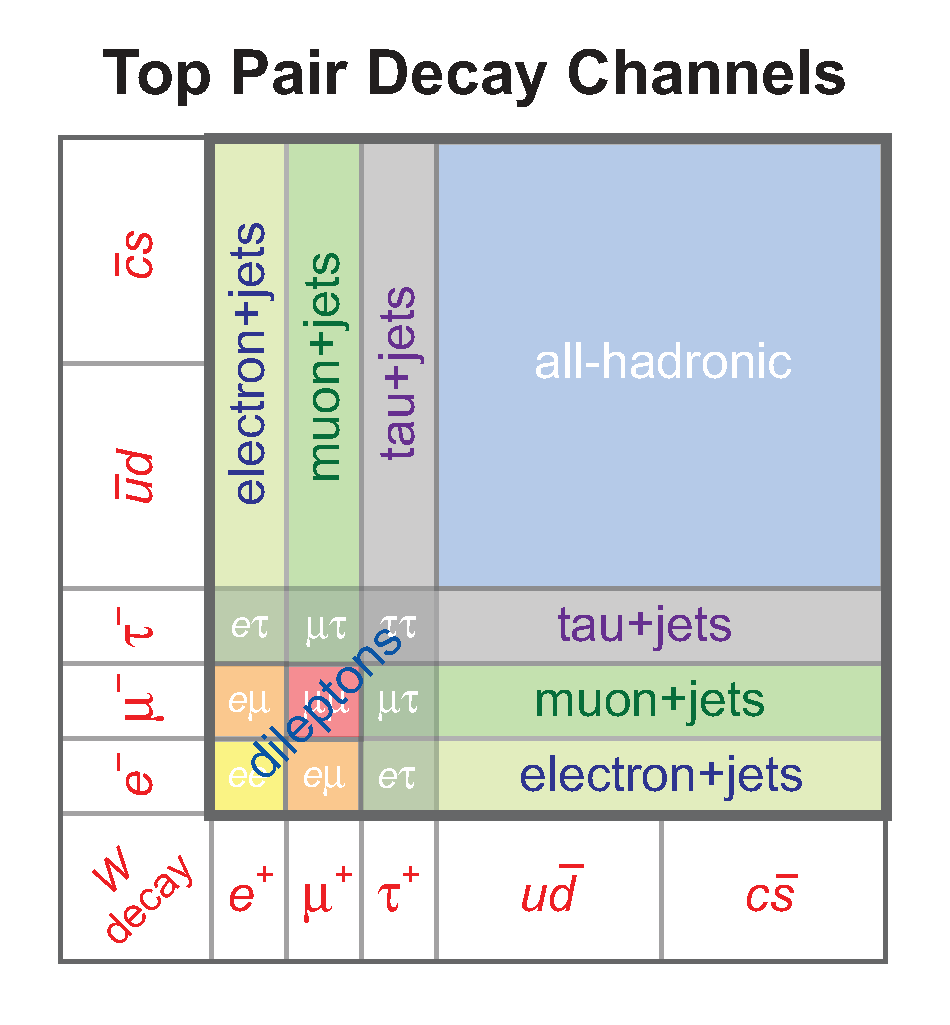
\includegraphics[width=0.5\textwidth]{Chapters/02_Theory/Images/top_pair_decay_channels.eps}\hfill
     \caption{Relative branching ratios of the \ttbar system}
     \label{fig:ttbar_branching_ratios}
\end{figure}

Gluon-gluon fusion contributes more at the LHC as a result of the gluon momentum fraction increasing at a
higher rate than that carried by the sea quarks which would be required to produce a top pair.